\subsection{Brukermedvirkning}
\label{chp: medvirkning}

Uttrykket \emph{brukermedvirkning} består av to deler, \emph{bruker} og \emph{medvikning}. Vi må derfor først være klar over at det finnes flere typer \emph{brukere}. Det kan være toppledelsen, som bruker systemets output i sine analyser og strategiske avgjørelser. Det kan være mellomledere som er ansvarlig for og overvåker avdelinger som bruker systemet. Til sist har vi de ansatte som bruker systemet i sitt daglige arbeid. Det vil være naturlig at alle disse forskjellige brukergruppene er involvert i utviklingsprosessen på noen måte. Toppledelsen må kanskje godkjenne prosjektet, og kan ha meninger om hva slags rapporter det skal generere. Mellomledelsen og andre ansatte kan bidra med innsikt i dagens arbeidsrutiner, problemer og workarounds samt kravspesifikasjoner, ønsker angående design og tesing. Når det kommer til \emph{medvirkning} må det understrekes at dette ikke er det samme som involvering, selv om de to uttrykkene ofte blir brukt om hverandre. i Cavaye (1995) finner vi definisjonene av (bruker)medvirkning og involvering som henholdsvis \emph{"a set of operations and activities performed by users"} i løpet av utviklingsprosessen, og \emph{"subjective psycological state"} som påvirker brukerenes forestillinger og dermed påvirker systemets suksess.

\noindent
Brukermedvikning finner vi i mange former og i mange nivåer. For å få et fullstendig bilde av medvirkningen, holder det derfor ikke å kun se på kun aktivitetene brukerene deltar i. som vi ser i tabell \ref{Beskrivelse av brukermedvirkning} kan vi beskrive medvirkningen ved help av flere attributter. Type medvirkning beskriver andelen av brukere som faktisk blir inkudert. Det er ikke alltid det lar seg gjøre å inkludere alle brukere i praksis. Da vil det være viktiv å etterstrebe å ha et representativt utvalg av disse med i prosessen. Graden av medvirkning viser til at brukere har forskjellig grad av ansvar gjennon sin medvirkning. Innholdet i medvirkningen refererer til det faktum at brukerene kan involveres i forskjellige aspekter av utviklingsprosessen. Det er veneligat brukere involveres i aktiviteter som forbereder det tekniske designet av systemet, men de kan også invilveres i det sosiale designet, som menneskelig og sosiale effekter systemet vil ha. Området medvirkningen angår vil variere gjennom de forskjellige fasene av utviklingsprosessen. Medvirkning fra brukerene er mer vanlig i forbindelse med å sette rammer for prosjektet, kravsspesifikasjon og testing enn gjennom selve utviklingen og kodingen av systemet. Medvikningen kan også være enten formell, med bruk av formelle grupper og team, og uformell, med mer tilfeldige diskusjoner og oppgaver. Til sist kan det være stor varisjon i hvor stor inflytelse brukerene har gjennom sin medvirkning. Dette kan variere helt fra at innspillene fra disse blir ignorer, og til at de virkelig tas seriøst. Dette betyr at det kan legges mye resureser i at brukerene skal ha sitt og si, men at virkning av disse beror på hvilken gard disse blir tatt hensyn til.

\begin{table}[H]
\caption{Beskrivelse av brukermedvikrning (hentet fra Cavaye (1995))}
%\centering
\begin{tabular}{c c}
\hline\hline
\textbf{Medvirkningsattributter} & \textbf{Mulige verdier} \\ [2ex]
\hline
& alle brukere \\[-1ex]
\raisebox{1.5ex}{Type} & representativt utvalg av brukere \\ [2ex]
\hline
& rådgivende \\ & signeringsansvar  \\
\raisebox{2ex}{Grad} & del av teamet \\ & fullt ansvar \\ [2ex]
\hline
& teknisk design \\
\raisebox{1.5ex}{Innhold} & sosialt og teknisk design \\ [2ex]
\hline
& prosjektdefinering  \\ & kravspesifikasjon  \\
\raisebox{2ex}{Område} & utvikling \\ & testing \\ [2ex]
\hline
& formell \\
\raisebox{1.5ex}{Formalitet} & uformell \\ [2ex]
\hline
& innspill ignorert \\
\raisebox{2ex}{Innflytelse} & bidrag tatt i betraktning  \\ & innspill tas seriøst \\
\hline
\end{tabular}
\label{Beskrivelse av brukermedvirkning}
\end{table} 

\noindent
I mange år ble det sett på som selvfølgelig at brukermedvirkning hadde en signinfikant positiv effekt på en eventuell suksess for et informsjonsystem. Empiriske studier er imidlertid ikke i stand til å bevise at det alltid er en slik årsakssammenheng \cite{Cavaye95}. Dermed ser det ut til at brukermedvirkning hverken er tilstrekkelig eller nødvendig for å garantere suksess for et informasjonsystem. Det er flere grunner til dette, både fra designer/utviklers side og fra brukerenes. For det første har forholdet mellom bruker og designer/utvikler stor innvirkning på effekten av medvirkningen. Forskjeller i bakgrunn, erfaringer og perspektiver kan føre til konflikter som igjen preger effekten av medvirkningen på en negativ måte. For det andre spiller det ingen rolle i hvor stor grad brukerene medvirker i prosessen dersom deres innspill blir ignorert. For det tredje vil de ansattes motstand mot endringen kunne resultere i ubrukte systemer, eller bevisst sabotasje av implementeringen og endringsprosessen. Som beskrevet i avsnitt \ref{chp: Motstand}, vil motstanden mot endring kunne reduseres ved god informasjon og involvering av de ansatte. Dette må ikke sees som en motsettning til Cavaye(1995)s påstand om at medvirkning ikke er en garanti for suksess. Dette fordi informasjon til og involvering av de ansatte ikke nødvendigvis behøver å inkludere medvirkning \cite{Cavaye95}, og fordi selv med medvirkning og innspill fra de ansatte er en ikke garantert å redusere motstanden tilstrekkelig.

\subsection{Deltagende design}
Interessen for deltagende design blir stadig større, og involvering av brukere tidlig i prosessen sees på som en god måte å blant annet sikre bedre kvalitet til sluttproduktet, gjensidig læring og bedring av arbeidsrutiner.

\noindent
Vi kan dele systemutvikling i tre aspekter: analyse, design og praksis. Det kan være vanskelig å kombinere alle tre samtidig, og tidligere ble det sett på som positivt om man greide å kombinere to av de. Mogensen og Trigg (1992) (kilde \cite{Mogensen92}) ser i sin artikkel på om det lar seg gjøre å kombinere alle tre aspekter (figur \ref{Challenge_PD}).

\begin{figure}[H]
\centering
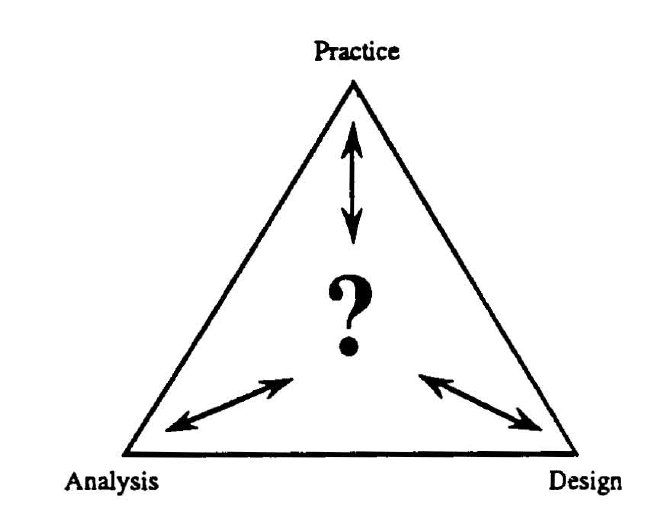
\includegraphics[scale=0.3]{Challenge_PD.jpg}
\caption{Hvordan kombinere alle?}
\label{Challenge_PD}
\end{figure}

\noindent
Ifølge \cite{Mogensen92} er det flere måter å oppnå større involvering av brukerene på. Én teknikk er fremtidsworkshops, der en ønsker en diskusjon rundt mulige fremtidige løsninger på nåværende problemer identifisert av brukerene selv. En annen teknikk er workshops hvor en bruker mock-ups og prototyper for å trigge diskusjonen om mulige fremtidige teknologier.  Uavhengig av valgt teknikk vil graden av relavans til dagens praksis være avgjørende for workshopens suksess. Felles for de to er at de tar i bruk kontekstuelle artefakter.

\noindent
Mogesen og Trigg (1992) konkluderer med at ved bruk av kontekstualiserte artefakter kan lede til nettopp et slikt ønsket samspill (figur \ref{Artifacts_PD}). De argumenterer for at bruk av artefakter under en workshop ikke bare gir innspill på design - deltagende design, men at de også kan trigge diskusjoner som gir utviklerene bedre innsyn i dagens praksis, problemer og workarounds - deltagende analyse. 

\noindent
Deltagende design på denne måten, med bruk av kontekstualiserte artefakter, gir derfor forskere/utviklere en dypere forståelse av hva som er problemområdene, og hvordan brukerene oppfatter dagens situasjon. Det gir også brukerene mulighet til å bli klar over egne arbeidsmetoder og workarounds.

\begin{figure}[H]
\centering
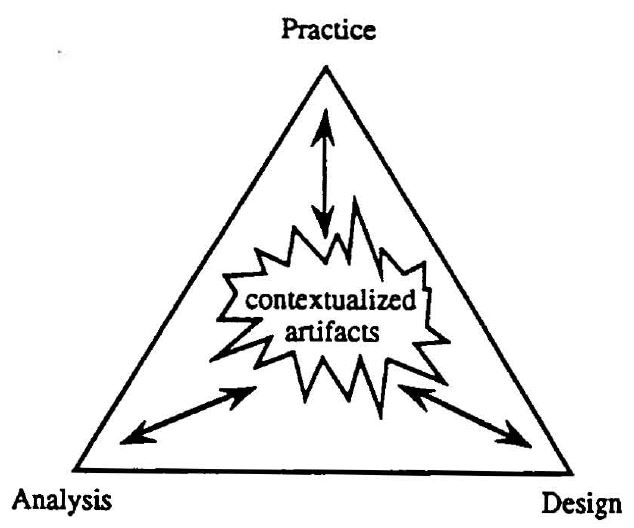
\includegraphics[scale=0.3]{Artifacts_PD.jpg}
\caption{Kontekstuelle artefakter støtter samspillet mellom de tre perspektivene}
\label{Artifacts_PD}
\end{figure}